\documentclass{beamer}
\usetheme{Antibes}
\usecolortheme{dolphin}
\usepackage{lmodern}
\usefonttheme{professionalfonts}
\usepackage{graphicx}
\graphicspath{{./figs/}}
\usepackage{siunitx}

\title{Scaling in DPD}
\author{Lu Lu}
\institute{DPD Club Meeting}
\date{Oct 8, 2015}

\begin{document}

\frame{\titlepage}

\section{DPD}

\begin{frame}
\frametitle{DPD}
\begin{gather}
    \frac{d \boldsymbol{r_i}}{dt} = \boldsymbol{v_i} \qquad \frac{d \boldsymbol{v_i}}{dt} = \boldsymbol{f_i} \\
    \boldsymbol{f_i} = \sum_{j \neq i} (\boldsymbol{F^C_{ij}} + \boldsymbol{F^D_{ij}} + \boldsymbol{F^R_{ij}}) \\
    \boldsymbol{F_{ij}^C} = \textcolor{red}{a_{ij}} \omega^C(r_{ij}) \boldsymbol{\hat{r}_{ij}} \\
    \boldsymbol{F_{ij}^D} = -\textcolor{red}{\gamma} \omega^D(r_{ij}) (\boldsymbol{\hat{r}_{ij} \cdot v_{ij}}) \boldsymbol{\hat{r}_{ij}} \\
    \boldsymbol{F_{ij}^R} = \textcolor{red}{\sigma} \omega^R(r_{ij}) \theta_{ij} \boldsymbol{\hat{r}_{ij}}
\end{gather}
Usually,
\begin{gather}
    \omega^C(r) = 1 - \frac{r}{\textcolor{red}{r_c}} \\
    \omega^D(r) = {[\omega^R(r)]}^2 = {(1 - \frac{r}{r_c})}^2
\end{gather}
\end{frame}

\begin{frame}
\frametitle{DPD}
How to choose $a$, $\gamma$, and $\sigma$?
\begin{itemize}
    \item scaling: different coarse grain level?
    \item match experimental parameters?
\end{itemize}
References
\begin{itemize}
    \item Groot \& Warren, J. Chem. Phys, 1997.
    \item Pivkin, J. Chem. Phys, 2006.
    \item Qiao \& He, J. Chem. Phys, 2008.
    \item Fuchslin, J. Chem. Phys, 2009.
\end{itemize}
\end{frame}

\section{Scaling}

\begin{frame}
\begin{columns}
\begin{column}{.5\textwidth}
    \begin{itemize}
        \item coarse graining level $\nu \equiv \frac{N_{phys}}{N}$
        \item scaling ratio $\phi \equiv \frac{\nu'}{\nu} = \frac{N}{N'}$
        \item mass of a DPD particle $m' = \phi m$
        \item $r'_c = \phi^{\frac{1}{d}}r_c$ \\
            $d$ is dimension
    \end{itemize}
\end{column}
\begin{column}{.5\textwidth}
    \begin{figure}
        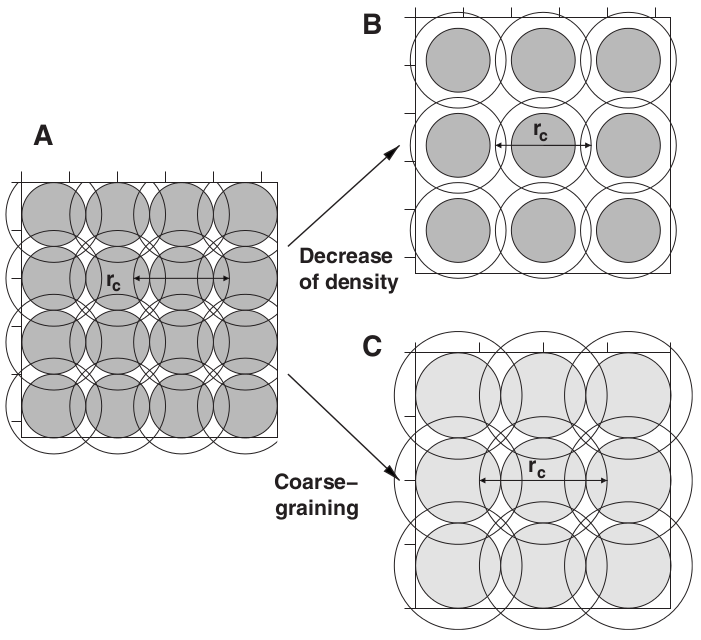
\includegraphics[width=\textwidth]{rc.png}
    \end{figure}
    B:\@ the mutual overlap of the soft particles is smaller.
\end{column}
\end{columns}
\end{frame}

\begin{frame}
Potential energy $U_0 = \sum_i^N \sum_{j>i} \frac{a}{2r_c} {(r_{ij}-r_c)}^2$ \\
For an isotropically compressed system, $L \rightarrow (1-\delta)L$, $\delta \ll 1$ \\
Assume $\Delta r_{ij}(\delta) = \delta r_{ij} + O(\delta^2)$
\begin{gather*}
    U_{\delta} = \sum_i^N \sum_{j>i} \frac{a}{2r_c} {(r_{ij} - \Delta r_{ij} (\delta) - r_c)}^2 \\
    \Delta U = U_{\delta} - U_0 = \sum_i^N \sum_{j>i} a(1- \frac{r_{ij}}{r_c})\delta r_{ij}
\end{gather*}
$\Delta U$ is invariant under scaling
\begin{gather*}
    \sum_i^N \sum_{j>i} a(1- \frac{r_{ij}}{r_c})\delta r_{ij} = \sum_i^{N'} \sum_{j>i}a'(1- \frac{r'_{ij}}{r'_c})\delta r'_{ij} \\
    a' = \phi^{1-\frac{1}{d}}a
\end{gather*}
\end{frame}

\begin{frame}
\begin{itemize}
\item $T' = T$
\item nondimensional $\tilde{a} = a \frac{r_c}{\epsilon}$ is invariant \\
    $\rightarrow$ energy unit $\epsilon'=\phi \epsilon$
\item $\epsilon=m\frac{{r_c}^2}{\tau^2}$ \\
    $\rightarrow$ time unit $\tau'=\phi^{\frac{1}{d}}\tau$
\item nondimensional $\tilde{\gamma} = \gamma \frac{r_c^2}{\epsilon \tau}$ is invariant \\
    $\rightarrow \gamma'=\phi^{1-\frac{1}{d}} \gamma$
\item $\sigma^2 = 2 k_B T \gamma$ \\
    $\rightarrow \sigma'=\phi^{1-\frac{1}{2d}}\sigma$
\end{itemize}
\end{frame}

\begin{frame}
\begin{columns}
\begin{column}{.4\textwidth}
    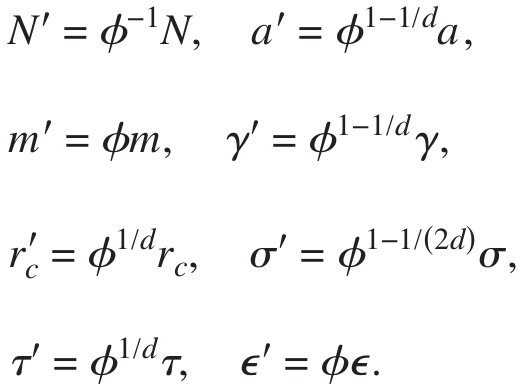
\includegraphics[width=\textwidth]{scaling.png}
\end{column}
\begin{column}{.6\textwidth}
    \begin{gather*}
        [\Delta \boldsymbol{v_i}]' = \sum_{j\neq i}\frac{[\boldsymbol{F_{ij}}]'}{m'} \Delta t' \\
        = \frac{\phi^{1-1/d}\phi^{1/d}}{\phi}\sum_{j\neq i}\frac{\boldsymbol{F_{ij}}}{m}\Delta t = \Delta \boldsymbol{v_i} \\
        \Delta \tilde{\boldsymbol{v_i}} = \Delta \boldsymbol{v_i}\frac{\tau}{r_c} \\
        \rightarrow \Delta \boldsymbol{\tilde{v}_i} = \Delta \boldsymbol{\tilde{v}}'_i \\
        \rightarrow \tilde{\boldsymbol{r}}(\tilde{t}) = \tilde{\boldsymbol{r}}'(\tilde{t}')
    \end{gather*}
\end{column}
\end{columns}
\end{frame}

\begin{frame}
at $\phi = 1$, $r_c =1, m=1, \rho=3, \gamma=4.5, \sigma=3$ \\
$a$ in [0, $\frac{50}{\phi^{2/3}}$] \\
$\phi$ = 1 (circles), 8 (squares), 125 (diamonds) \\
BC: reflective walls
\begin{figure}
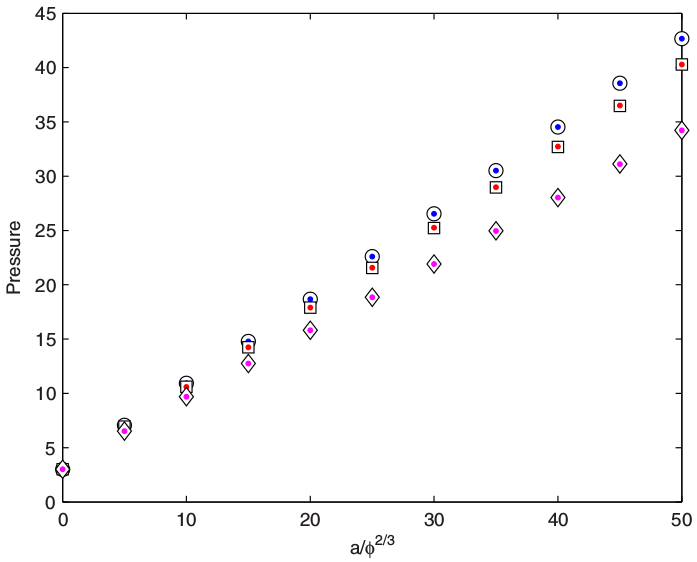
\includegraphics[height=.7\textheight]{p.png}
\end{figure}
\end{frame}

\begin{frame}
periodic BC \\
$a$ in [0, $\frac{100}{\phi^{2/3}}$], $\phi$ in [1, 125]
\begin{figure}
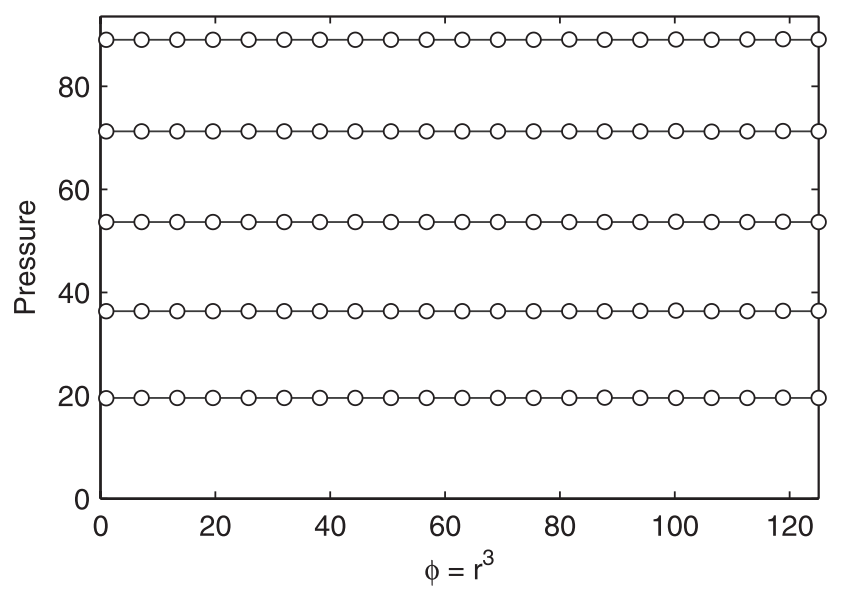
\includegraphics[height=.7\textheight]{p2.png}
\end{figure}
\end{frame}

\section{a}

\begin{frame}
\frametitle{Compressibility and $a$}
\begin{equation*}
\kappa^{-1}={(\frac{1}{nk_BT\kappa_T})}_{phys}=\frac{1}{\textcolor{red}{\nu} k_BT}{(\frac{\partial p}{\partial \rho})}_T
\end{equation*}
$n$: number density of physical molecules, for water, \SI{3.337e28}{m^{-3}}
\begin{gather*}
    p = \rho k_B T + \frac{2\pi}{3}\rho^2 \int_0^1 rf(r)g(r)r^2dr \\
    \rightarrow p = \rho k_B T + \alpha a \rho^2 \qquad \alpha = 0.101 \pm 0.001 \\
    \rightarrow a = k_BT \frac{\kappa^{-1}\nu - 1}{2\alpha \rho} \qquad \rho \geq 3r_c^{-3}
\end{gather*}
\end{frame}

\section{Conclusions}

\begin{frame}
\frametitle{Conclusions}
Map parameters from one DPD system to another
\begin{figure}
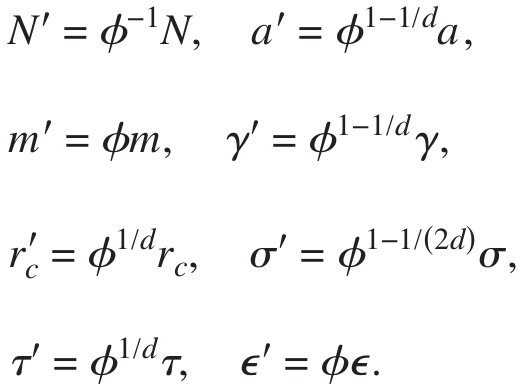
\includegraphics[height=.4\textheight]{scaling.png}
\end{figure}
Determine $a$ by compressibility
$$a = k_BT \frac{\kappa^{-1}\nu - 1}{2\alpha \rho}$$
\end{frame}

\end{document}
